\section{Top Quark and Higgs Boson Decay}
\label{problem_and_app}

In the LHC, two proton beams are accelerated close to the speed of light in opposite directions, set to collide inside a specific particle detector. This head-on collision triggers a chain reaction of decaying particles, and most of the final particles react with the detector, recording relevant data. One of the experiments being conducted at the ATLAS detector aims to study the top quark and Higgs boson properties\cite{Higgs}. Figure \ref{fig:ttbar} presents the schematic representation of the top quark decay (addressed as the \ttbar system).

\begin{figure}[!htp]
	\begin{center}
		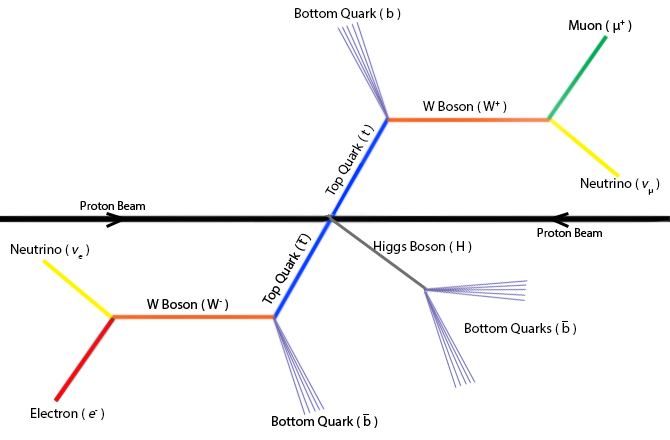
\includegraphics[scale=0.45]{images/ttbar_higgs.png}
		\caption{Schematic representation of the \ttbar system and Higgs boson decay.}
		\label{fig:ttbar}
	\end{center}
\end{figure}

The ATLAS detector can record the characteristics of the bottom quarks, detected as a jet of particles, and leptons (muon and electron). Neutrinos do not interact with the detector, so, their characteristics are not recorded. Since the top quark reconstruction requires the neutrinos, their characteristics are analytically determined with the known information of the system, through a kinematical reconstruction. However, the \ttbar system may not have a possible reconstruction: the reconstruction has a degree of certainty associated, which determines its quality.

The amount of bottom quark jets and leptons detected may vary among events, due to other reactions occurring alongside the top quark decay. As represented in figure \ref{fig:ttbar}, two jets and two leptons are needed to reconstruct the \ttbar system, but the captured data for an event may contain many more of these particles. For the kinematical reconstruction every combination of two jets and two leptons must be evaluated and only the most accurate reconstruction of each event is considered.

If the \ttbar system has a possible reconstruction the Higgs boson is reconstructed from the two bottom quark jets that it decays to. This adds two more jets to the event information to test in both kinematical and Higgs reconstructions. The Higgs reconstruction uses the jets that did not provide the most accurate \ttbar system. The overall quality of the event processing depends on the quality of both reconstructions.

The ATLAS detector has an experimental resolution of $\pm1\%$ for each measured value. This error is propagated into the \ttbar system and Higgs reconstructions, affecting their accuracy. To improve the quality of the reconstructions several random variations are applied to the measured particles parameters, with a maximum magnitude of $|1\%|$. The quality of the reconstructions and the application execution time is directly proportional to the amount of variations performed per combination. The goal is to do as many variations as possible within a reasonable time frame.

To reconstruct the \ttbar system and Higgs boson a data analysis application was developed, the \tth. The application flow is presented in figure \ref{fig:flow}. Each event data on an input file is individually loaded into a single global state, shared between the data analysis code and the LipMiniAnalysis toolbox\footnote{The LipMiniAnalysis toolbox provides a skeleton to several data analysis applications under study in the Portuguese LIP institution, a CERN partner in the ATLAS experiment.}, and it is overwritten every time a new event is loaded. The event is then submitted to a series of cuts, which filters events that are not suited for reconstruction. When an event reaches the cut 20 the \ttbar system and Higgs boson are reconstructed in the function \ttDilepKinFit, which is expected to be the most computing demanding. If the \ttbar system reconstruction fails, the current combination is discarded and the next is processed. If an event has a possible reconstruction it passes the final cut and its final information is stored.

\begin{figure}[!htp]
	\begin{center}
		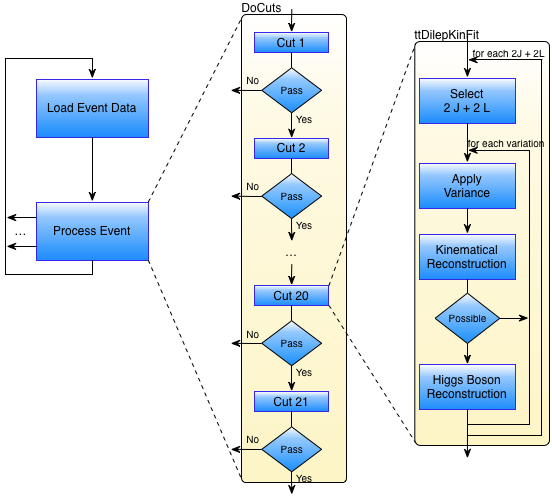
\includegraphics[scale=0.5]{images/graf_abstract_flow_with_kinfit.png}
		\caption{Schematic representation for the \tth application flow.}
		\label{fig:flow}
	\end{center}
\end{figure}

The application also depends on the ROOT framework\footnote{ROOT \cite{ROOT} is a C++ framework produced by CERN  to help the development of particle daa analsis code, by implementing specific features.} for part of the functionalities used in the reconstructions and for result output and visualisation. The code from both ROOT and the LipMiniAnalysis toolbox cannot be modified as many data analysis applications depend on them.
